\subsection{Translation and ribosomal synthesis}

Lastly, we turn our attention to the process of synthesizing new proteins,
translation. These processes stand as good candidates for defining the growth
limit as the synthesis of new proteins relies on the generation of ribosomes,
themselves proteinaceous molecules. As we will see in the coming sections of
this work, this poses a "chicken-or-the-egg" problem where the synthesis of
ribosomes requires ribosomes in the first place. 

We will begin our exploration of protein translation in the same spirit as we
have in previous sections -- we will draw order-of-magnitude estimates based on
our intuition and relying on literature studies and will compare these estimates
to the observed data. In doing so, we will estimate both the absolute number of
ribosomes necessary for replication of the proteome as well as the synthesis of
amino-acyl tRNAS. In the closing sections, we will explore the details of
ribosome biogenesis in granular detail, ultimately presenting a quantitative
model tying ribosome abundance to the concentration of amino acids as well as
the state of chromosome replication.

\subsubsection{tRNA synthetases}
We begin by first estimating the number of tRNA ligases in \textit{E. coli}
needed to convert free amino-acids to polypeptide chains. At a modest growth
rate of $\approx$ 5000 s, \textit{E. coli} has roughly 3$\times$10$^6$ proteins
per cell (BNID: 115702; \cite{milo2010}). Assuming that the typical protein is 
on the order of $\approx$ 300 amino acids in length (BNID: 100017;
\cite{milo2010}), we can estimate that a total of $\approx$ 10$^9$ amino acids
are stitched together by peptide bonds.  

How many tRNAs are needed to facilitate this remarkable number of amino acid
delivery events to the translating ribosomes? It is important to note that tRNAs
are recycled after they've passed through the ribosome and can be recharged with
a new amino acid, ready for another round of peptide bond formation. While some
\textit{in vitro} data exists on  the turnover of tRNA in \textit{E. coli} for
different  animo acids, we can make a reasonable estimate by comparing the
number of amino acids to be  polymerized to cell division time. Using our
stopwatch of 5000 s and 10$^9$ amino acids, we arrive at a requirement of
$\approx$ 2 $\times$ 10$^5$ tRNA molecules. This estimate is in line with
experimental measurements of $\approx$ 3 $\times$ 10$^5$ per cell (BNID: 108611,
\cite{milo2010}), suggesting we are on the right track.

There  are many processes which go into synthesizing a tRNA and ligating it
with the appropriate amino acids. As we covered  in the previous section, there
appear to be more than enough RNA polymerases per cell to synthesize the needed
pool of tRNAs. Without considering the many ways in which amino acids can be
scavenged or synthesized \textit{de novo}, we can explore ligation the as a potential rate limiting
step. The enzymes which link the correct amino acid to the tRNA, known as tRNA
synthetases or tRNA ligases, are incredible in their proofreading of substrates
with the incorrect amino acid being ligated once out of every $10^4$ to $10^5$
times (BNID: 103469, \cite{milo2010}). This is due in part to the consumption of
energy  as well as a multi-step pathway to ligation. While the rate at which
tRNA is ligated is highly dependent on the identity of the amino acid, it is
reasonable to state that the typical tRNA synthetase has charging rate of
$\approx$ 20 AA per tRNA synthetase per second (BNID: 105279, \cite{milo2010}).

Combining these estimates together, as shown schematically in
\FIG{protein_synthesis}(A), yields an estimate of $\approx$ 10$^4$ tRNA
synthetases per cell with a division time of 5000 s. This point estimate is in
very close agreement with the observed number of synthetases (the sum of all 20
tRNA synthetases in \textit{E. coli}). This estimation strategy seems to
adequately describe the observed growth rate dependence of the tRNA synthetase copy
number (shown as the grey line in \FIG{protein_synthesis}(B)), suggesting that
the copy number scales with the cell volume. 

In total, the estimated and observed $\approx$ 10$^4$ tRNA synthetases occupy
only a meager fraction of the total cell proteome, around 0.5\% by abundance. It
is reasonable to assume that if tRNA charging was a rate limiting process, cells
would be able to increase their growth rate by devoting more cellular resources
to making more tRNA synthases. As the synthesis of tRNAs and the corresponding
charging can be highly parallelized, we can argue that tRNA charging is not a
rate limiting step in cell division, at least for the growth conditions explored
in this work. 

\subsubsection{Protein synthesis}
With the number of tRNA synthetases accounted for, we now consider the abundance
of the protein synthesis machines themselves, ribosomes. Ribosomes are enormous
protein/rRNA complexes that facilitate the peptide bond formation between amino
acids in the correct sequence as defined by the coding mRNA. Before we examine
the synthesis of the ribosome proteins and the limits that may place on the
observed bacterial growth rates, let's consider replication of the cellular
proteome.  

As described in the previous section, \textit{E. coli} consists of $\approx$
3$\times$10$^6$ proteins at a growth rate of $\approx$ 5000 s. If we again
assume that each protein is composed of $\approx$ 300 amino acids and each amino
acid is linked together by one peptide bond, we arrive at an estimate that the
cellular proteome consists of $\approx$ 10$^10$ peptide bonds. While the rate at
which ribosomes translates is well known to have a growth rate dependence
\cite{dai2018} and is a topic which we discuss in detail in the coming sections.
However, for the purposes of our order-of-magnitude estimate, we can make the
approximation that translation occurs at a rate of $\approx$ 15 amino acids per
second per ribosome (BNID: 100233, \cite{milo2010}). Under this approximation
and assuming a division time of 5000 s, we can arrive at an estimate of
$\approx$10$^4$ ribosomes are needed to replicate the cellular proteome, shown
in \FIG{protein_synthesis}(B). This point estimate, while glossing over
important details such as chromosome copy number and growth-rate dependent
translation rates, proves to be notably accurate when compared to the
experimental observations (\FIG{protein_synthesis}(B)). 

\subsection{Translation as a growth-rate limiting step}
Thus far in our work, the general back-of-the-envelope estimates have been 
reasonably successful in explaining what sets the scale of absolute protein copy
number. In many cases, these estimates can be adapted to consider a continuum of
growth rates in lieu of a single 5000 s point estimate, the details of which are
described in the Supplemental Information. A recurring theme we have relied on
is the ability of the cell to parallelize different processes to transport or
synthesize the required amount of the corresponding biomolecule. For example, we
saw in our example of \textit{E. coli} grown on different carbon sources that
expression of particular transporters can be induced, often producing more
than needed acquire enough carbon to build new cell mass (\FIG{carbon_transport}(B)). In
examining replication of the DNA, we described how cells can replicate multiple
copies of the chromosome at any given time, permitting growth rates faster than
the limit at which the chromosome can be faithfully replicated.  As a final
example, we showed how increasing the gene dosage of the rRNA operons is
necessary to produce enough rRNA to form functional ribosomes. However, when it
comes to ribosome biogenesis, namely the translation of ribosomal proteins,
such parallelization is not possible, suggesting that translation may be a key
factor determining the cellular growth rate. 

Optimal resource allocation and the role of ribosomal proteins have been an
area of intense quantitative study over the last decade by Hwa and others
\citep{scott2010, hui2015}. From the perspective of limiting growth, our
earlier estimate of rRNA highlighted the necessity for multiple copies of
rRNA genes in order to make enough rRNA. For \textit{E. coli}'s fastest
growth rates at 2 hr$^{-1}$, the additional demand for rRNA is further
supported by parallelized DNA replication and increased rRNA gene dosage.
This suggests the possibility that synthesis of ribosomes might be rate
limiting. While the transcriptional demand for the ribosomal proteins is
substantially lower than rRNA genes, since proteins can be translated from
relatively fewer mRNA, other ribosomal proteins like the translation
elongation factor EF-Tu also present a substantial burden. For EF-Tu in
particular, it is the most highly expressed protein in \textit{E. coli} and
is expressed from multiple gene copies, \textit{tufA} and \textit{tufB}.

\begin{figure}
    \begin{fullwidth}
    \centering{
        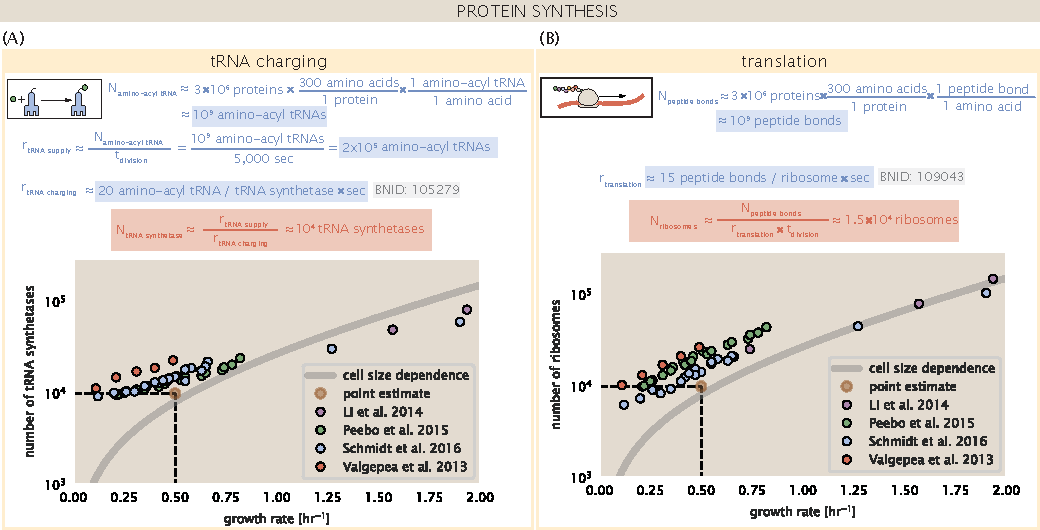
\includegraphics{main_figs/fig8_protein_synthesis.pdf}
        \caption{\textbf{Estimation of the required tRNA synthetases and
        ribosomes.} (A) Estimation for the
        number of tRNA synthetases that will supply the required amino acid
        demand. The sum of all tRNA synthetases copy numbers are plotted as a
        function of growth rate ([ArgS], [CysS], [GlnS], [GltX], [IleS], [LeuS],
        [ValS], [AlaS]$_2$, [AsnS]$_2$, [AspS]$_2$, [TyrS]$_2$, [TrpS]$_2$,
        [ThrS]$_2$, [SerS]$_2$, [ProS]$_2$, [PheS]$_2$[PheT]$_2$, [MetG]$_2$,
        [lysS]$_2$, [HisS]$_2$, [GlyS]$_2$[GlyQ]$_2$). (B) Estimation of the
        number of ribosomes required to synthesize 10$^9$ peptide bonds with an
        elongation rate of 15 peptide bonds per second. The
        average abundance of ribosomes is plotted as a function of growth rate.
        Our estimated values are shown for a growth rate of 0.5 hr$^{-1}$.
        Grey lines correpsond to the estimated complex abundance calculated at
        different growth rates. See Supplemental Information XX for a more
        detail description of this calculation.}
    \label{fig:protein_synthesis}
    }
    \end{fullwidth}
\end{figure}

To gain some intuition into how translation may set the speed limit for bacterial
growth, we again consider the total number of peptide bonds that must be synthesized,
$N_\text{AA}$. Noting that cell mass grows exponentially \citep{godin2010}, we
can compute the number of amino acids to be polymerized as \begin{equation}
N_\text{AA} = \frac{r_t R}{\lambda}, \end{equation} where $\lambda$ is the cell
growth rate in s$^{-1}$, $r_t$ is the maximum translation rate in amino acids
per second, and $R$ is the average ribosome copy number per cell. Knowing the
number of peptide bods to be formed permits us to compute the
translation-limited growth rate as \begin{equation}
\lambda_\text{translation-limited} = \frac{r_t R}{N_\text{AA}}.
\end{equation}

Alternatively, since $N_{AA}$ is related to the total protein mass through the
molecular weight of each protein, we can also consider the growth rate in terms
of the fraction of the total proteome mass that is dedicated to ribosomal
protein mass. By making the approximation that an average amino acid has a
molecular weight of 110 Da (see \FIG{ribosome_limit}(A)), we can rewrite the
growth rate as,

\begin{equation}
\lambda_{\textrm{translation-limited}} \approx \frac{r_t}{L_R}  \Phi_R,
\label{eq:translation_limit_growth_rate}
\end{equation}
where $L_R$ is the total length in amino acids that make up a ribosome, and
$\Phi_R$ is the ribosomal mass fraction. This is plotted as a function of
ribosomal fraction $\Phi_R$ in \FIG{ribosome_limit}(A), where we take $L_R
\approx$ 7500 aa, corresponding to the length in amino acids for all ribosomal
subunits of the 50S and 30S complex (BNID: 101175, \citep{milo2010}). This
formulation assumes that the cell can transcribe the required amount of rRNA,
which appears reasonable for \textit{E. coli}, allowing us to
consider the inherent limit on growth set by the ribosome.

The growth rate defined by Equation \ref{eq:translation_limit_growth_rate}
reflects mass-balance under steady-state growth and has long provided a
rationalization to the apparent linear increase in \textit{E. coli}'s
ribosomal content as a function of growth rate \citep{Goldberger1979,
scott2010}. For our purposes, there are several important consequences of
this trend. Firstly, we note there is a maximum growth rate of $\lambda
\approx 6 \text{hr}^{-1}$, or doubling time of about 7 minutes (dashed line).
This growth rate can be viewed as an inherent maximum growth rate due to the
need for the cell to double the cell's entire ribosomal mass. Interestingly,
this limit is independent of the absolute number of ribosomes and is simply
given by time to translate an entire ribosome, $L_R/ r_t$. As shown in
\FIG{ribosome_limit}(B), we can reconcile this with the observation that in
order to double the average number of ribosomes, each ribosome must produce a
second ribosome. Unlike DNA replication or rRNA transcription, this is a
process that cannot be parallelized.

\begin{figure}
  \begin{fullwidth}
        \centering{
            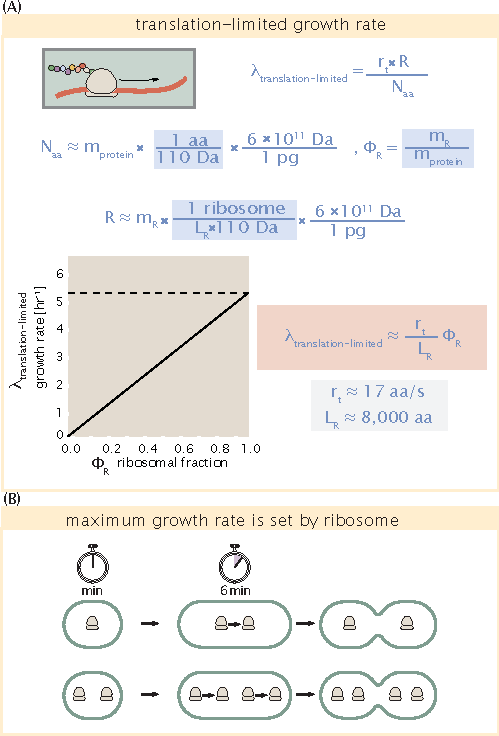
\includegraphics{main_figs/fig7_ribosome_growth_limit.pdf}
            \caption{\textbf{Translation-limited growth rate.} (A) Here we
            consider the translation-limited growth as a function of ribosomal
            fraction. By mass balance, the time required to double the entire
            proteome ($N_{AA}$ /$r_t$) sets the translation-limited
            growth rate, $\lambda_{\textrm{translation-limited}}$. Here $N_{aa}$
            is effectively the number of peptide bonds that must be translated,
            $r_t$ is the translation elongation rate, and $R$ is the number of
            ribosomes. This can also be re-written in terms of the ribosomal
            mass fraction $\Phi_R = m_R$ / $m_{\textrm{protein}}$, where $m_R$
            is the total ribosomal mass and $m_{\textrm{protein}}$ is the mass
            of all proteins in the cell. $L_R$ refers to the summed length of
            the ribosome in amino acids.
            $\lambda_{\textrm{translation-limited}}$ is plotted as a function of
            $\Phi_R$ (solid line). (B) The dashed line in part (A) identifies a
            maximum growth rate that is set by the ribosome. Specifically, this
            growth rate corresponds to the time required to  translation an
            entire ribosome, $L_R/ r_t$ . This is a result that is independent
            of the number of ribosomes in the cell as shown schematically here.
            (C)
            }
        \label{fig:ribosome_limit}
        }
  \end{fullwidth}
\end{figure}

For reasonable values of $\Phi_R$, between about 0.1 - 0.3 \citep{scott2010},
the maximum growth rate is in line with experimentally reported growth rates
around 0.5 - 2 hr$^{-1}$. Importantly, in order for a cell to increase their
growth limit they \textit{must} increase their relative ribosomal abundance.
This can be achieved by either synthesizing more ribosomes or reducing the
fraction of non-ribosomal proteins. Reduction of non-ribosomal proteins is not a
straightforward task since (as we have found throughout our estimates) doubling
a cell requires many other enzymes and transporters. Increasing the absolute
ribosomal abundance in \textit{E. coli} will be limited by the number of rRNA
operons.

Here we again return to rRNA synthesis, but here consider the maximum rRNA that can
be produced at different growth rates.

[expand on.]
